\section{Results}
\label{sec:results}
\begin{figure}[htbp]
\vspace{-.3cm}
   \centering
    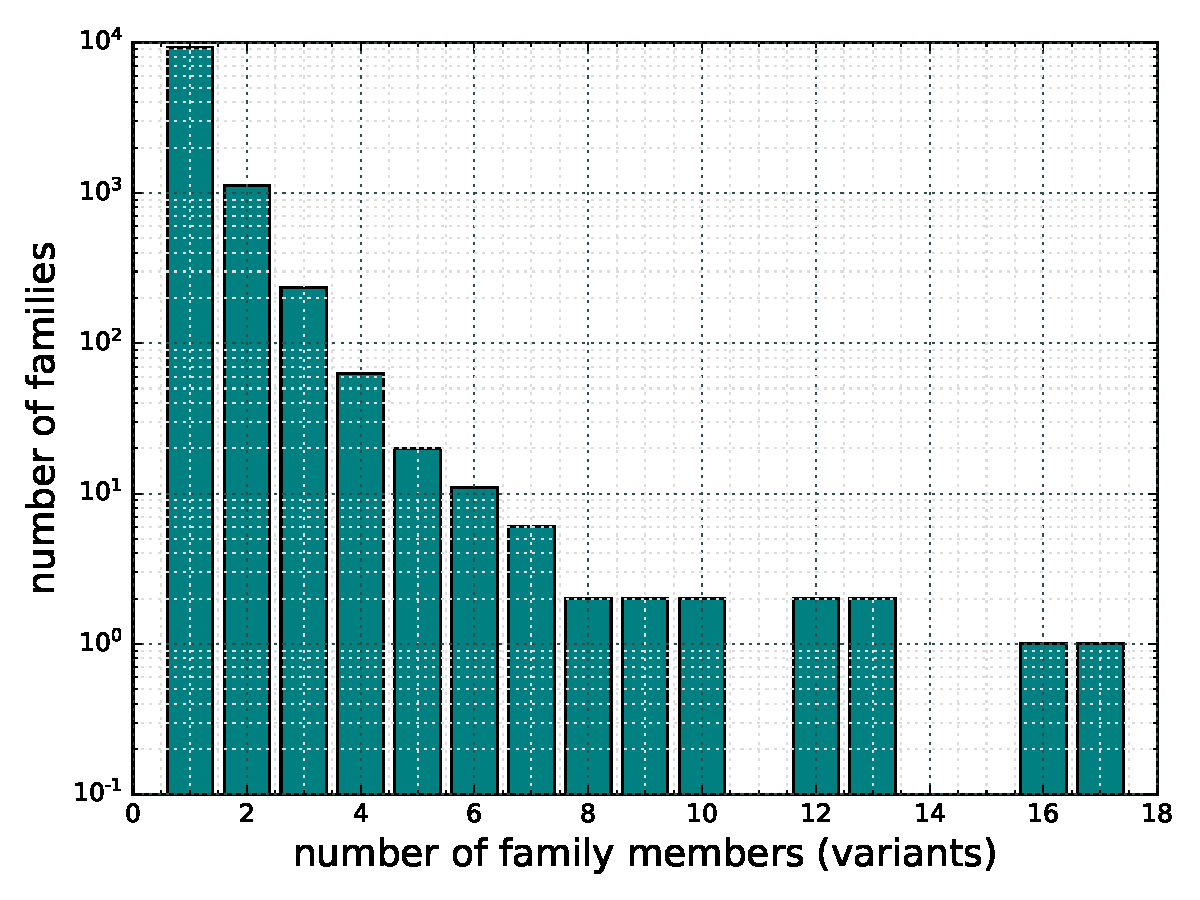
\includegraphics[scale=0.4]{figures/variants.pdf}
    \caption{Family size (number of variants in a family).}
    \label{fig:variants}
\end{figure}

\noindent
\textit{RQ0}: \textbf{How prevalent are software families?}

With this first RQ, we aim to determine if software families exist in software ecosystems. In the \js ecosystem we discovered 12,813 variants of the mainline and a total of 10,743 software families. In Figure~\ref{fig:variants} we present the distribution of the software families. On the y-axis we have the number of families and on the x-axis we have the number of variants in the families. For example, the first bar tells us that there are 9,280 families that contain only one variant. We also observe one family each containing as many as 16 and 17 variants, respectively. The results of RQ0 give us confidence that indeed software families exist in software ecosystems.

\begin{figure}[htbp]
\vspace{-.3cm}
   \centering
    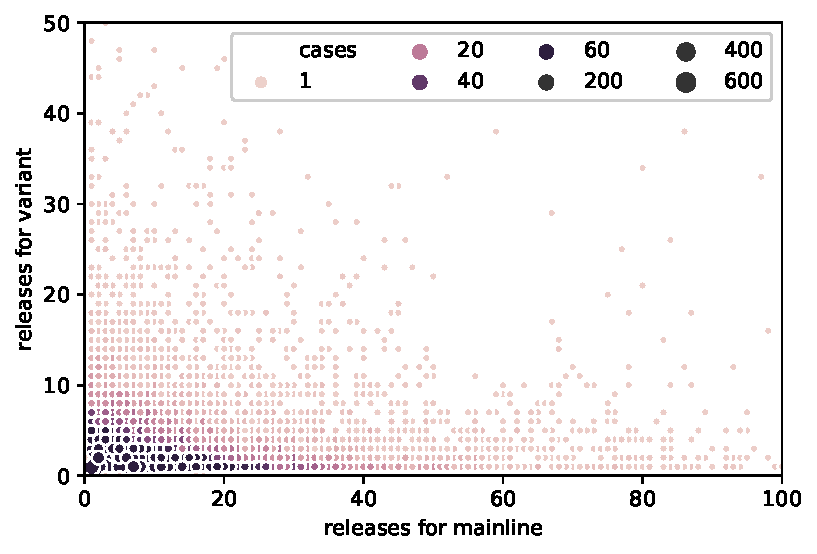
\includegraphics[scale=0.6]{figures/benevolj_releases.pdf}
    \caption{The distribution of the mainline versus variant package releases.}
    \label{fig:releases}
\end{figure}

\textit{RQ1}: \textbf{The distribution of package releases for mainlines versus variants.}

With this second RQ, we aim to ascertain if the mainlines and the variants are continuously maintained. 
In Figure~\ref{fig:releases} we present a scatter plot showing the distribution of releases for the variants versus the releases for the mainlines. 
On the x-axis we have the number of releases for the mainlines and on the y-axis we have the number of releases for the variants. 
The color of the data points in the graph represent the number cases for the mainlines\,/\,variants. 
For example, the data points on the top left of the graph tell us that there are some variants that have more releases compared to their mainline counterparts. 
This implies the variants are being maintained more than their mainline counterparts.
The data points on the bottom right tell us that there are a number of mainlines having many releases compared to their variant counterparts. 
Overall, we observe more mainlines being maintained compared to their variant counterparts.
However, we also observe a significant amount of variants being maintained. 
This is interesting since developers variants did not make a one off package distribution; they are continuously distributing new releases of their package. 

\begin{figure}[htbp]
\vspace{-.3cm}
   \centering
    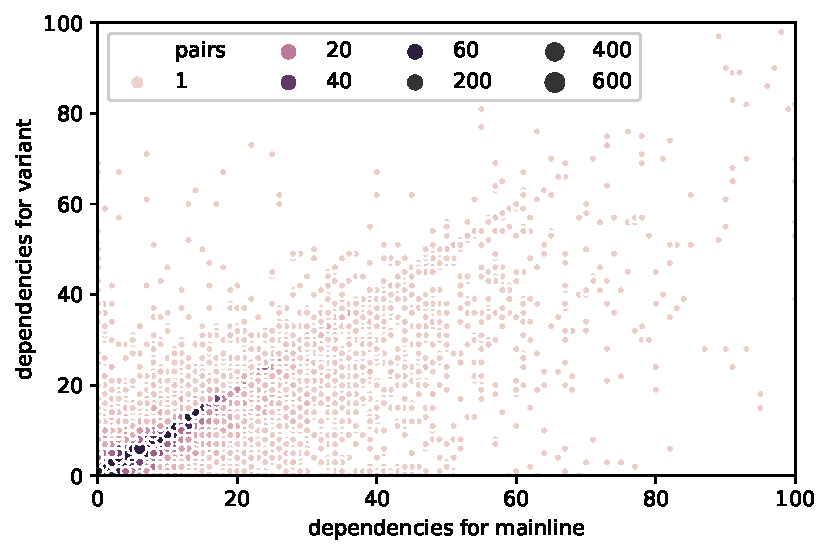
\includegraphics[scale=0.6]{figures/benevolj_dependencies.pdf}
    \caption{The distribution of the mainline versus variant package dependencies.}
    \label{fig:dependencies}
\end{figure}


\textit{RQ2}: \textbf{The distribution of package dependencies for the mainlines versus variants.}

With this RQ, we want to ascertain the frequency of package dependencies on other packages for the mainlines and the variants in the software families. 
In Figure~\ref{fig:dependencies} we present a scatter plot showing the distribution of the package dependencies of the variants versus the dependencies of the mainline.
On the x-axis we have the number of dependencies of the mainline. 
On the y-axis we have the number of dependencies of the variant.
The color of the data points in the graph represent the number cases for the mainlines\,/\,variants.
For example, on the top right of the graph we see a few scattered points single case variants telling us that there are a few variants that have many dependencies compared to the mainline counterparts.
We also see many scattered single case mainlines having many dependencies compared to their variant counterparts. 
Overall, we observe the mainlines having more dependencies compared to their variant counterparts.

\begin{figure*}%
    \centering
    \subfloat[Packages]{{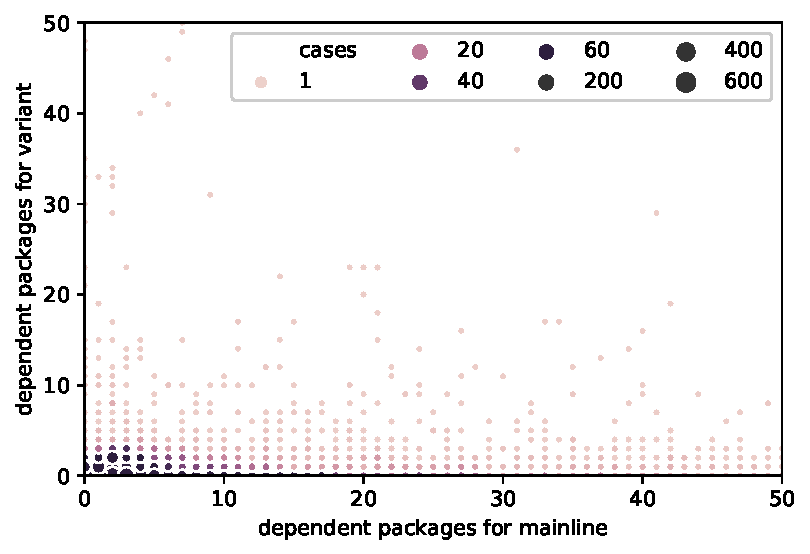
\includegraphics[width=8cm]{figures/dependents} }}%
    \qquad
    \subfloat[Projects]{{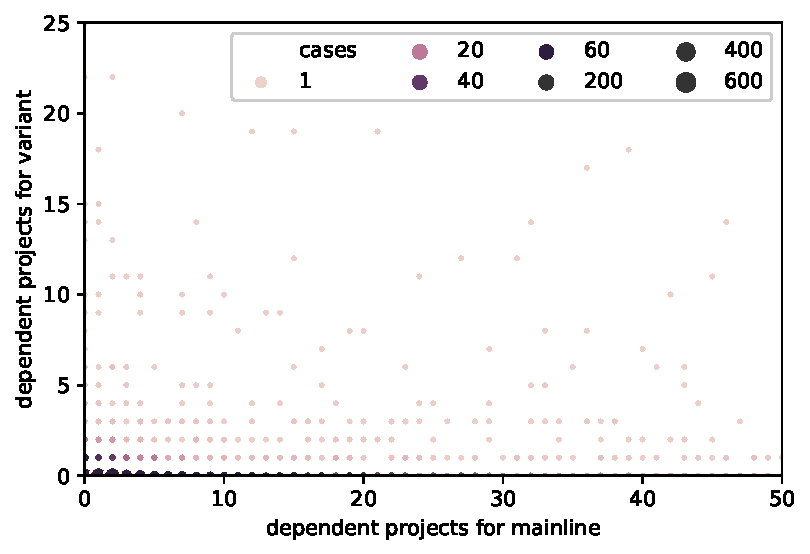
\includegraphics[width=8cm]{figures/benevolj_projects} }}%
    \caption{Distribution of dependent packages and dependent projects for the mainline versus variants.}%
    \label{fig:packages_and_projects}%
\end{figure*}


\begin{figure*}%
    \centering
    \subfloat[ Mainlines]{{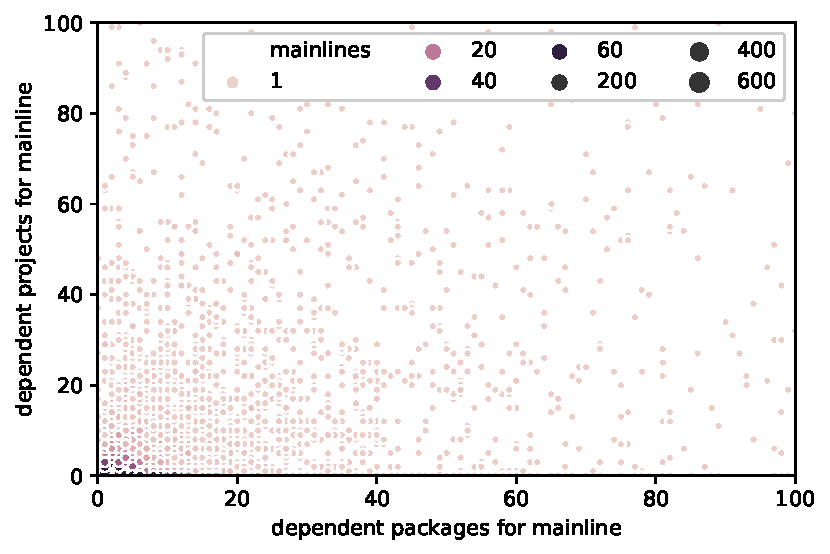
\includegraphics[width=8cm]{figures/benevolj_dependents_mainline.pdf} }}%
    \qquad
    \subfloat[ Variants]{{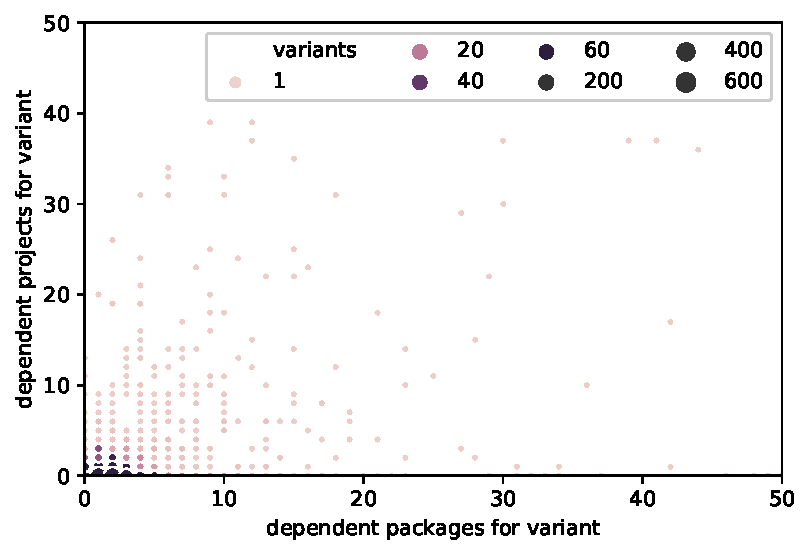
\includegraphics[width=8cm]{figures/benevolj_dependents_variant.pdf} }}%
    \caption{Distribution of dependent packages versus dependent projects for mainlines and variants.}%
    \label{fig:mainline_variants_packages}%
\end{figure*}

\textit{RQ3}: \textbf{The distribution of dependent packages and projects of the mainlines and variants.}

In this RQ we are interesting in observing if other packages\,/\,projects in the ecosystem depend on the variants.
In Figure~\ref{fig:packages_and_projects} we present the scatter plots showing the distribution of the dependent packages (Figure~\ref{fig:packages_and_projects}-(a)) and dependent projects (Figure~\ref{fig:packages_and_projects}-(b)) for the variants versus mainlines.
The x-axes represent the number of dependent packages for the mainline and number of dependent projects for the variants, respectively.
The y-axes represent the number of dependent packages for the variants and number of dependent projects for the variants, respectively.
The color of the data points in the graph represent the number cases for the mainlines\,/\,variants.
Looking at Figure~\ref{fig:packages_and_projects}-(a), we observe that most of the data points are concentrated on the x-axis. 
This implies that there are very many mainline variants having many dependent packages compared to their variant counterparts.
We observe the same trend for the dependent projects in Figure~\ref{fig:packages_and_projects}-(b).
In both Figure~\ref{fig:packages_and_projects}-(a) and Figure~\ref{fig:packages_and_projects}-(b), we observe that most variants have $<10$ dependent packages\,/\,projects. 
This is still interesting since it implies that some developers do depend on the variants as opposed to their mainlines counterparts offering similar functionality.
